
\documentclass[letterpaper, reqno,12pt]{article}
\usepackage[margin=1.0in]{geometry}
\usepackage{color,latexsym,amsmath,amssymb}
\usepackage{fancyhdr}
\usepackage{amsthm}
\usepackage[linesnumbered,lined,boxed,commentsnumbered]{algorithm2e}
\usepackage{dsfont}
\usepackage{graphicx}
\usepackage{hyperref}
\usepackage{lmodern}
\usepackage[numbers]{natbib}
\usepackage{listings}% http://ctan.org/pkg/listings
\lstset{
  basicstyle=\ttfamily,
  columns=fullflexible,
  mathescape
}
\usepackage{enumitem}
\usepackage{tikz}

\allowdisplaybreaks

\newcommand{\RR}{\mathbb{R}}
\newcommand{\CC}{\mathbb{C}}
\newcommand{\ZZ}{\mathbb{Z}}
\newcommand{\QQ}{\mathbb{Q}}
\newcommand{\NN}{\mathbb{N}}
\newcommand{\PP}{\mathop{{}\mathbb{P}}}
\newcommand{\EE}{\mathop{{}\mathbb{E}}}
\newcommand{\mynote}[3][red]
  {{\color{#1} \fbox{\bfseries\sffamily\scriptsize#2}
  {\small$\blacktriangleright$\textsf{\emph{#3}}$\blacktriangleleft$}}~}
\newcommand{\yp}[1]{\mynote{YP}{#1}}
\newcommand\mycommfont[1]{\ttfamily\textcolor{blue}{#1}}
\SetCommentSty{mycommfont}
\DeclareMathOperator{\conv}{conv}
\DeclareMathOperator{\charcone}{char.cone}
\DeclareMathOperator{\STAB}{STAB}
\DeclareMathOperator{\Down}{Down}
\DeclareMathOperator{\lca}{lca}
\DeclareMathOperator{\LPO}{LPO}
\DeclareMathOperator{\OPT}{\mathit{OPT}}
\DeclareMathOperator{\LHS}{LHS}
\DeclareMathOperator{\RHS}{RHS}
\DeclareMathOperator{\tr}{tr}
\DeclareMathOperator{\vol}{vol}
\DeclareMathOperator{\argmin}{arg\,min}
\DeclareMathOperator{\argmax}{arg\,max}
\DeclareMathOperator{\poly}{poly}
\DeclareMathOperator{\Span}{span}
\begin{document}
\pagenumbering{arabic}
\title{\Large Randomization in Recent Progress on Traveling Salesman Problem}
\author{Yuchong Pan\thanks{MIT, \href{mailto:yuchong@mit.edu}{yuchong@mit.edu}.}}
\date{\today}
\newtheorem{theorem}{Theorem}[section]
\newtheorem{lemma}[theorem]{Lemma}
\newtheorem{corollary}[theorem]{Corollary}
\newtheorem{proposition}[theorem]{Proposition}
\newtheorem{fact}[theorem]{Fact}
\theoremstyle{definition} \newtheorem{definition}[theorem]{Definition}
\maketitle
%

\section{Introduction}

\begin{quote}
  It belongs to the most seductive problems in combinatorial optimization, thanks to a blend of complexity, applicability, and appeal to imagination.

  --- Schrijver \cite{schrijver2003combinatorial}
\end{quote}

The (metric) traveling salesman problem (TSP) is one of the most appealing yet challenging problems in combinatorial optimization: given a set $V$ of $n$ vertices and symmetric pairwise costs $c : V \times V \to \RR_+$ which satisfy the triangle inequality, find a minimum cost tour that visits each vertex exactly once. One of the most classical linear programming relaxations for the TSP is formulated by Dantzig, Fulkerson and Johnson \cite{dantzig1954solution}, known as the \emph{subtour elimination LP}:
\begin{alignat*}{4}
  & \text{minimize} \qquad & \sum_{u, v \in V} x_{\{ u, v \}} c(u, v) \\
  & \text{subject to} \qquad & \sum_{\{ u, v \} \in \delta(S)} x_{\{ u, v \}} &\geq 2 && \qquad \forall S \subsetneq V, S \neq \emptyset \\
  & & \sum_{\{ u, v \} \in \delta(\{ v \})} x_{\{ u, v \}} &= 2 && \qquad \forall v \in V \\
  & & x_{\{ u, v \}} &\in [0, 1] && \qquad \forall u, v \in V
\end{alignat*}

In 1976 and 1978, Christofides \cite{christofides1976worst} and Serdyukov \cite{serdyukov1978nekotorykh} independently devised a simple deterministic algorithm, now known as the Christofides-Serdyukov algorithm and given in Algorithm \ref{alg:christofides-serdyukov}, which gives a $3/2$-approximation to the metric TSP. Wolsey \cite{wolsey1980heuristic} extended the analysis of Christofides and Serdyukov to show an upper bound of $3/2$ on the integrality gap of the subtour elimination LP. On the negative side, there exists a family of instances of the metric TSP whose integrality ratios converge to $4/3$, thereby giving a lower bound of $4/3$ on the integrality gap. One such family of instances is called the \emph{envelope graphs}, illustrated in Figure \ref{fig:envelope}. It is conjectured that the integrality gap of the subtour elimination LP is $4/3$.

\begin{algorithm}[h]
  $T \leftarrow \text{a minimum spanning tree of $G$}$ \\
  $O \leftarrow \{ v \in V : \deg_T(v) \text{ is odd} \}$ \\
  $M \leftarrow \text{a minimum-weight perfect matching in $G[O]$}$ \\
  find a Eulerian tour in $T \cup M$ \\
  shortcut repeated vertices in the Eulerian tour to form a Hamiltonian tour
  \caption{The Christofides-Serdyukov algorithm, given an undirected graph $G = (V, E)$ and edge costs $c : \EE \to \RR_+$ which satisfy the triangle inequality.}
  \label{alg:christofides-serdyukov}
\end{algorithm}

\begin{figure}[h]
  \centering
  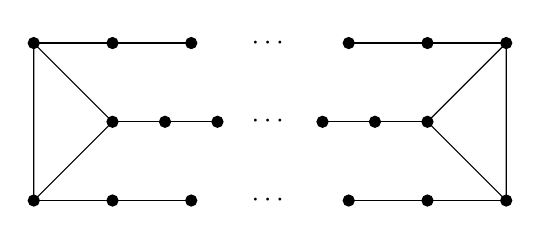
\begin{tikzpicture}
    \draw[fill=black] (0, 0) circle (2pt);
    \draw[fill=black] (0, -2) circle (2pt);
    \draw[fill=black] (1, -1) circle (2pt);
    \draw[fill=black] (5, -1) circle (2pt);
    \draw[fill=black] (6, 0) circle (2pt);
    \draw[fill=black] (6, -2) circle (2pt);
    \draw[fill=black] (1, 0) circle (2pt);
    \draw[fill=black] (2, 0) circle (2pt);
    \draw[fill=black] (4, 0) circle (2pt);
    \draw[fill=black] (5, 0) circle (2pt);
    \draw[fill=black] (1, -2) circle (2pt);
    \draw[fill=black] (2, -2) circle (2pt);
    \draw[fill=black] (4, -2) circle (2pt);
    \draw[fill=black] (5, -2) circle (2pt);
    \draw[fill=black] (1.667, -1) circle (2pt);
    \draw[fill=black] (2.333, -1) circle (2pt);
    \draw[fill=black] (3.667, -1) circle (2pt);
    \draw[fill=black] (4.333, -1) circle (2pt);
    \draw (0, 0) -- (0, -2) -- (1, -1) -- cycle;
    \draw (5, -1) -- (6, 0) -- (6, -2) -- cycle;
    \draw (0, 0) -- (2, 0);
    \draw (4, 0) -- (6, 0);
    \draw (1, -1) -- (2.333, -1);
    \draw (3.667, -1) -- (5, -1);
    \draw (0, -2) -- (2, -2);
    \draw (4, -2) -- (6, -2);
    \node at (3, 0) {$\cdots$};
    \node at (3, -1) {$\cdots$};
    \node at (3, -2) {$\cdots$};
  \end{tikzpicture}
  \caption{A family of instances matching the $4/3$ lower bound of the subtour elimination LP, where each of the three horizontal paths consists of $k$ edges, and the cost of each edge is $1$. An optimal Hamiltonian tour takes $4k + 4$ edges. A feasible fractional solution to the subtour elimination LP is given by setting $x_e = 1$ on each edge $e$ on the three horizontal paths, and $x_e = 1/2$ on each of the other edges. Hence, the integrality ratio equals $(4k + 4)/(3k + 3)$, which approaches $4/3$ as $k \to \infty$.}
  \label{fig:envelope}
\end{figure}

$3/2$ had remained the best known approximation ratio and the best known upper bound on the integrality gap for almost half a century, until the recent breakthrough of Karlin, Klein and Oveis Gharan \cite{karlin2021slightly, karlin2021slightlyig}, which improves both bounds by a small constant $\varepsilon > 10^{-36}$. Their works combine the Christofides-Serdyukov algorithm and randomization --- instead choosing a minimum spanning tree, their algorithm samples a spanning tree from the \emph{max-entropy distribution} with marginals matching the optimal solution to the subtour elimination LP. More recently, Gupta et al.\ \cite{gupta2021matroid} further improve the Christofides-Serdyukov framework in the special case where the subtour elimination LP has optimal half-integral solutions, by randomizing between the max-entropy distribution and a distribution based on matroid intersection, using an idea of Haddadan and Newman \cite{haddadan2019towards}.

The approach of the max-entropy distribution of spanning trees was first introduced in the work of Oveis Gharan, Saberi and Singh \cite{gharan2011randomized} on the special case of the metric TSP where the metric is defined by shortest path distances in an undirected graph. In this note, we study how randomization, especially the max-entropy distribution of spanning trees, helps break the $3/2$ barrier in the Christofides-Serdyukov algorithm.

\section{Preliminaries}

\subsection{Strongly Rayleigh Distributions}

As we shall see, the max-entropy distribution on spanning trees is a special case of \emph{strongly Rayleigh} distributions. Therefore, we first define strongly Rayleigh distributions and study their general properties.

A new theme in computer science and combinatorics that has emerged in the past two decades is to encode a complicated mathematical object (e.g., a probability distribution or a combinatorial object) in a complex multivariate polynomial, and properties of this polynomial (e.g., zeros of the polynomial) help reason properties of the underlying object. It turns out that strongly Rayleigh distributions are closely related to \emph{real stable} polynomial.

\begin{definition}
  Let $\mu$ be a probability distribution on spanning trees in a graph $G$. The \emph{generating polynomial} of $\mu$ is defined to be
  $$ p(z) = \sum_{T \in \mathcal T} \mu(T) \prod_{e \in E(T)} z_e, $$
  where $\mathcal T$ is the set of all spanning trees in $G$. We say that $\mu$ is \emph{strongly Rayleigh} (or \emph{SR}) if $p$ is \emph{real stable} (i.e., $p(z) \neq 0$ whenever $z \in \mathcal H^n$, where $\mathcal H = \{ w \in \CC : \Im(z) > 0 \}$).
\end{definition}

\begin{definition}
  For $\lambda \in \RR_+^E$, we say that a probability distribution $\mu$ on spanning trees in a graph $G$ is \emph{$\lambda$-uniform}, or \emph{weighted uniform}, if
  $$ \mu(T) \propto \prod_{e \in E(T)} \lambda_e. $$
\end{definition}

\begin{theorem}[\cite{borcea2009negative}]
  Any weighted uniform distribution on spanning trees in a graph $G$ is strongly Rayleigh.
\end{theorem}

Recall that the \emph{entropy} of a probability distribution $\mu : \mathcal T \to \RR_+$ on spanning trees in a graph $G$, where $\mathcal T$ is the set of all spanning trees in $G$, is $\sum_{T \in \mathcal T} -\mu(T) \log \mu(T)$.

\begin{definition}
  The \emph{max-entropy distribution} $\mu^* : \mathcal T \to \RR_+$ of spanning trees in a graph $G = (V, E)$ with respect to some given marginals $z \in \RR^E$ is the optimal solution to the following convex program:
  \begin{alignat*}{4}
    & \text{minimize} \qquad & \sum_{T \in \mathcal T} \mu(T) \log \mu(T) \\
    & \text{subject to} \qquad & \sum_{\substack{T \in \mathcal T \\ e \in E(T)}} \mu(T) &= z_e && \qquad \forall e \in E \\
    & & p(T) &\geq 0 && \qquad \forall T \in \mathcal T
  \end{alignat*}
\end{definition}

Given a vector $z \in \RR^E$ in the \emph{spanning tree polytope} of a graph $G = (V, E)$, i.e.,
\begin{alignat*}{2}
  z(E) &= |V| - 1 \\
  z(E(S)) &\leq |S| - 1 && \qquad \forall S \subset V \\
  z_e &\geq 0 && \qquad \forall e \in E
\end{alignat*}
there exist various algorithms that find an ``approximate'' max-entropy distribution that preserves some given marginals $z \in \RR^E$ approximately, e.g., the multiplicative weight update algorithm \cite{asadpour2017log}, interior point methods \cite{sebHo2014shorter}, and the ellipsoid method \cite{asadpour2017log}. For simplicity, we call such a distribution the ``max-entropy distribution,'' and assume that it preserves the given marginals exactly.

\begin{theorem}[\cite{asadpour2017log}] \label{thm:max-entropy}
  Let $z \in \RR^E$ be a vector in the spanning tree polytope of a graph $G = (V, E)$. For any $\varepsilon > 0$, a vector $\lambda \in \RR_+^E$ can be found such that for all $e \in E$,
  $$ \sum_{\substack{T \in \mathcal T \\ e \in E(T)}} \mu(T) \leq (1 + \varepsilon) z_e, $$
  where the running time is polynomial in $|V|$, $\log (1/\min_{e \in E} z_e)$ and $\log (1/\varepsilon)$.
\end{theorem}

Now, we study several important properties of strongly Rayleigh distributions that are used in recent randomized algorithms for the metric TSP. The first ones are the closure properties of strongly Rayleigh distributions, which follow from a set of linear operators that preserve the real stability of a polynomial. We omit the background and refer interested readers to a seminal series of papers by Borcea and Br\"and\'en \cite{borcea2009lee,borcea2009lee2,borcea2010multivariate}.

\begin{theorem}[\cite{borcea2009negative}] \label{thm:closure}
  Strongly Rayleigh distributions are closed under the following operations:
  \begin{itemize}[itemsep=0pt, topsep=5pt]
    \item {\bf Projection.} For any strongly Rayleigh distribution $\mu$ on spanning trees in a graph $G = (V, E)$, and any $F \subset E$, the \emph{projection} of $\mu$ onto $F$ is the measure $\mu|_F : 2^F \to \RR_+$ defined by
    $$ \mu|_F(A) = \sum_{\substack{S \subset E \\ S \cap F = A}} \mu(S). $$
    \item {\bf Conditioning.} For any $e \in E$, conditioning on $e \in T$ or on $e \not \in T$ preserves the strongly Rayleigh property.
    \item {\bf Truncation.} For any strongly Rayleigh distribution $\mu$ on subsets of a ground set $E$, and for any $k \in \{ 0, \ldots, |E| \}$, the \emph{truncation} of $\mu$ to $k$ is the measure $\mu_k: 2^E \to \RR_+$ defined by
    $$ \mu_k(A) = \left\{
      \begin{array}{ll}
        \mu(A)/\sum_{S \subset E : |S| = k} \mu(S), & \text{if $|A| = k$}, \\
        0, & \text{otherwise}.
      \end{array}
    \right. $$
  \end{itemize}
\end{theorem}

By the fundamental fact that the roots of a univariate polynomial come in conjugate pairs, one can easily characterize univariate real stable polynomials by its real-rootedness. This characterization is particularly useful for applications on proabability theory and randomized algorithms because it has a close connection to the sum of Bernoulli random variables.

\begin{theorem}[\cite{gharan2011randomized}] \label{thm:sum-of-bernoulli}
  Let $\mu$ be a strongly Rayleigh distribution on spanning trees in a graph $G = (V, E)$. Let $T \sim \mu$. Let $S \subset E$. Let $X_S = |S \cap T|$. Then
  $$ X_S \sim \sum_{i = 1}^{|S|} Y_i, $$
  where $Y_1, \ldots, Y_{|S|}$ are independent Bernoulli random variables with success probabilities $p_i$, and $\sum_{i = 1}^{|S|} p_i = \EE[X_S]$.
\end{theorem}

Strongly Rayleigh distributions also enjoy the virtues of the following three properties, namely log-concavity of the rank sequence, negative association, and stochastic dominance.

\begin{definition}
  The \emph{rank sequence} of a probability distribution $\mu$ on subsets of a ground set $E$ is a sequence $q_0, \ldots, q_{|E|}$, where $q_i = \PP_{S \sim \mu}[|S| = i]$ for all $i \in \{ 0, \ldots, |E| \}$.
\end{definition}

\begin{definition}
  A sequence $a_0, \ldots, a_m$ is \emph{log-concave} if $a_k^2 \geq a_{k - 1} a_{k + 1}$ for all $k \in [m - 1]$.
\end{definition}

\begin{theorem}[\cite{hardy1952inequalities,darroch1964distribution,borcea2009negative}] \label{thm:log-concave}
  The rank sequence of any strongly Rayleigh distribution is log-concave.
\end{theorem}

\begin{definition}
  A function $f : 2^E \to \RR$ is \emph{non-decreasing} if $f(A) \leq f(B)$ for any $A \subset B \subset E$, and \emph{non-increasing} if $-f$ is non-decreasing.
\end{definition}

\begin{definition}
  A probability distribution $\mu$ on subsets of a ground set $E$ is \emph{negatively associated} if
  $$ \EE_\mu[f] \EE_\mu[g] \geq \EE_\mu[fg], $$
  for any non-decreasing functions $f$ and $g$ that are disjointly supported.
\end{definition}

Feder and Mihail \cite{feder1992balanced} proved that uniform distributions on balanced matroids (in particular, on spanning trees in a graph) have negative association. Borcea et al. \cite{borcea2009negative} proved that strongly Rayleigh distributions have the strongest form of negative association.

\begin{theorem}[\cite{borcea2009negative}] \label{thm:negative-assoc}
  Any strongly Rayleigh distributions is negatively associated.
\end{theorem}

Roughly, stochastic dominance says that truncation on larger numbers increases the probability of the underlying elements and \emph{upward closed} events defined on them.

\begin{definition}
  A probability event $\mathcal A \subset 2^E$ for some ground set $E$ is \emph{upward closed} if for any $A \subset B \subset E$, if $A \in \mathcal A$, then $B \in \mathcal A$.
\end{definition}

\begin{definition}
  Given two probability distributions $\mu$ and $\nu$, we say that $\mu$ \emph{stochastically dominates} $\nu$, written $\nu \preccurlyeq \mu$, if $\nu(\mathcal A) \leq \mu(\mathcal A)$ for any upward closed probability event $\mathcal A$.
\end{definition}

\begin{theorem}[\cite{borcea2009negative}] \label{thm:stochastic-dominance}
  If $\mu$ is a strongly Rayleigh distribution on subsets of a ground set $E$, and if $\mu_k, \mu_{k + 1}$ are well-defined for some $k \in \{ 0, \ldots, |E| - 1 \}$, then $\mu_k \preccurlyeq \mu_{k + 1}$.
\end{theorem}

Lastly, we shall use a theorem of Hoeffding \cite{hoeffding1956distribution} to compute the degree distribution of a vertex in the analysis of the algorithm:

\begin{theorem}[\cite{hoeffding1956distribution}] \label{thm:hoeffding}
  For any Bernoulli random variables $B_1, \ldots, B_n$ with success probabilities $p_1, \ldots, p_n$ and any $g : \RR \to \RR$, $\EE[g(B_1 + \ldots + B_m)]$ is minimized when $p_1, \ldots, p_m \in \{ 0, p, 1 \}$ for some fixed $p$.
\end{theorem}

\subsection{$O$-Joins}

The notion of $O$-joins\footnote{These are typically referred to as $T$-joins in the literature. However, since we use $T$ to denote a (random) spanning tree, we call these $O$-joins.} is motivated by the Chinese postman problem, and extends the notion of matchings. For conciseness we omit the motivation of $O$-joins and refer interested readers to the survey of Frank \cite{as1994survey} and the book of Schrijver \cite{schrijver2003combinatorial}.

\begin{definition}
  Let $G = (V, E)$ be an undirected graph. Let $O \subset V$. A subset $J \subset E$ is called an \emph{$O$-join} if
  $$ T = \left\{ v \in V : \left|\delta_J(v)\right| \text{ is odd} \right\}. $$
\end{definition}

Note that if an $O$-join exists, then $O$ is even. More precisely, $G$ has an $O$-join if and only if $|K \cap O|$ is even for each component $K$ of $G$. The following observation is important and helps understand the motivation of $O$-joins.

\begin{proposition}
  Let $G = (V, E)$ be an undirected graph. Let $O \subset V$. Then $J$ is an $O$-join if and only if $J$ is the union of edge-disjoint cycles and $|O|/2$ paths connecting disjoint pairs of vertices in $O$.
\end{proposition}

\begin{definition}
  Let $G = (V, E)$ be an undirected graph. Let $O \subset V$. The \emph{$O$-join polytope} $P_\text{$O$-join}(G)$ is defined to be the convex hull of the characteristic vectors of $O$-joins in $G$. The \emph{up-hull} $P_\text{$O$-join}^\uparrow(G)$ of the $O$-join polytope is defined to be
  $$ P_\text{$O$-join}^\uparrow(G) = P_\text{$O$-join} + \RR_+^E = \left\{ y \in \RR^n : \exists x \in P_\text{$O$-join}, y \geq x \right\}. $$
\end{definition}

In their seminal paper, Edmonds and Johnson \cite{edmonds1973matching} characterized the up-hull of the $O$-join polytope.

\begin{theorem}[\cite{edmonds1973matching}]
  The polyhedron $P_\text{$O$-join}^\uparrow(G)$ is determined by
  \begin{alignat*}{2}
    \sum_{e \in \delta(S)} y_e &\geq 1 && \qquad \forall S \subset V, |S \cap O| \text{ odd} \\
    y_e &\geq 0 && \qquad \forall e \in E
  \end{alignat*}
\end{theorem}

\begin{corollary} \label{cor:min-o-join}
  For any undirected graph $G = (V, E)$ with edge costs $c : E \to \RR_+$, and for any $O \subset V$ with $|O|$ even, the minimum cost of an $O$-join equals the optimal solution to the following LP:
  \begin{alignat*}{4}
    & \text{minimize} \qquad & \sum_{e \in E} c(e) y_e \\
    & \text{subject to} \qquad & \sum_{e \in \delta(S)} y_e &\geq 1 && \qquad \forall S \subset V, |S \cap O| \text{ odd} \\
    & & y_e &\geq 0 && \qquad \forall e \in E
  \end{alignat*}
  Hence, the optimal solution to the LP is always integral.
\end{corollary}

\section{A Randomized Rounding Scheme for the Graph TSP}

In this section, we present the randomized rounding algorithm of Oveis Gharan, Saberi and Singh \cite{gharan2011randomized} for a special case, called the \emph{graph TSP}, of the metric TSP where the metric is a \emph{graph matric}.

\begin{definition}
  A metric $c : V \times V \to \RR_+$ on a ground set $V$ is a \emph{graph metric} if there exists an unweighted undirected graph $G = (V, E)$, where $c$ is the shortest path metric of $G$.
\end{definition}

We present the algorithm in Algorithm \ref{alg:oss}. Let $x$ be an optimal solution to the subtour elimination LP. Let $z = (1 - 1/n) x$ (so $z$ is in the spanning tree polytope). Let $G = (V, E, z)$ be the weighted support graph of $z$. To illustrate the role randomness, especially strongly Rayleigh distributions on spanning trees, plays in this algorithm and to simplify the argument, we assume that $G$ has no proper minimum cuts with respect to $z$, i.e., $\sum_{e \in \delta(S)} x_e \geq 2 + \varepsilon_0$ for some $\varepsilon_0 > 0$. In the general case, we exploit the structure of near-minimum-cuts called the \emph{deformable polygon representation} developed by a series of papers by Bencz\'ur and Goemans \cite{benczur1995representation, benczur1995structure, benczur1997cut, benczur2008deformable}.

\begin{algorithm}
  solve the subtour elimination LP to obtain an optimal solution $x$ \\
  $z \leftarrow (1 - 1/n) x$ \\
  compute the max-entropy distribution $\mu$ with marginals $z$ \CommentSty{(Theorem \ref{thm:max-entropy})} \\
  sample $T \sim \mu$ \\
  $O \leftarrow \{ v \in V: \deg_T v \text{ odd} \}$ \\
  find a minimum cost $O$-join $J$ \CommentSty{(Corollary \ref{cor:min-o-join})} \\
  \Return{$T \cup J$}
  \caption{A randomized rounding algorithm for the graph TSP by Oveis Gharan, Saberi and Singh \cite{gharan2011randomized}.}
  \label{alg:oss}
\end{algorithm}

\begin{theorem}[\cite{gharan2011randomized}] \label{thm:main}
  Suppose that there exists $\varepsilon_0 > 0$ such that $\sum_{e \in \delta(S)} x_e \geq 2 + \varepsilon_0$ for any proper cut $S \subset V$. Then for any cost function $c : E \to \RR_+$ satisfying the triangle inequality, the approximation ratio of Algorithm \ref{alg:oss} is $3/2 - \Omega(\varepsilon_0)$.
\end{theorem}

Let $\OPT$ be the optimal value to the subtour elimination LP. Since $T \sim \mu$ and since $\mu$ preserves marginals $z$,
\begin{align*}
  \EE_{T \sim \mu}\left[\sum_{e \in E(T)} c(e)\right] &= \EE_{T \sim \mu}\left[\sum_{e \in E} c(e) \mathds 1[e \in E(T)]\right] = \sum_{e \in E} c(e) \EE_{T \sim \mu}[\mathds 1[e \in E(T)]] \\
  &= \sum_{e \in E} c(e) \PP_{T \sim \mu}[e \in E(T)] = \sum_{e \in E} c(e) z_e \\
  &= \left(1 - \frac{1}{n}\right) \sum_{e \in E} c(e) x_e = \left(1 - \frac{1}{n}\right) \OPT.
\end{align*}
Hence, to prove Theorem \ref{thm:main}, it suffices to show that $\EE_{T \sim \mu}[\sum_{e \in J} c(e)] \leq (1/2 - \Omega(\varepsilon_0)) \OPT$.

\begin{theorem}[\cite{gharan2011randomized}] \label{thm:o-join}
  Suppose that there exists $\varepsilon_0 > 0$ such that $\sum_{e \in \delta(S)} x_e \geq 2 + \varepsilon_0$ for any proper cut $S \subset V$. For any cost function $c : E \to \RR_+$ satisfying the triangle inequality,
  $$ \EE_{T \sim \mu}\left[\sum_{e \in J} c(e)\right] \leq \left(\frac{1}{2} - \Omega\left(\varepsilon_0\right)\right) \OPT. $$
\end{theorem}

\subsection{Motivation}

To motivate the proof of Theorem \ref{thm:o-join}, we first show that $\sum_{e \in J} c(e) \leq \OPT/2$ for any spanning tree $T$ in $G$, hence reproducing the approximation ratio of $3/2$ as in the Christofides-Serdyukov algorithm. It suffices to construct a vector $y$ in the up-hull of the $O$-join polytope.

\begin{proposition} \label{prop:half}
  Let $T$ be a spanning tree in $G$. Let $O$ be the set of odd degree vertices in $T$. Let $J$ be a minimum cost $O$-join. Then
  $$ \sum_{e \in J} c(e) \leq \frac{\OPT}{2}. $$
\end{proposition}

\begin{proof}
  Let $y \in \RR_+^E$ be defined by $y_e = x_e/2$ for all $e \in E$. We show that $y \in P_\text{$O$-join}(G)^\uparrow$. Since $|O|$ is even, then $S \subset V$ with $|S \cap O|$ odd implies that $S$ is proper. For any $S \subsetneq V$ with $S \neq \emptyset$, since $\sum_{e \in \delta(S)} x_e \geq 2$ , then
  $$ \sum_{e \in \delta(S)} y_e = \sum_{e \in \delta(S)} \frac{x_e}{2} = \frac{1}{2} \sum_{e \in \delta(S)} x_e \geq \frac{1}{2} \cdot 2 = 1. $$
  Hence, $y \in P_\text{$O$-join}(G)^\uparrow$. Since $J$ is a minimum cost $O$-join, then by Corollary \ref{cor:min-o-join},
  $$ \sum_{e \in J} c(e) \leq \sum_{e \in E} c(e) y_e = \sum_{e \in E} c(e) \frac{x_e}{2} = \frac{1}{2} \sum_{e \in E} c(e) x_e = \frac{\OPT}{2}. $$
  This completes the proof.
\end{proof}

In the proof of Proposition \ref{prop:half}, we have indeed proved that $\sum_{e \in \delta(S)} y_e \geq 1$ for any non-singleton cut $S$ in $G$. However, in order to have a feasible solution to the minimum cost $O$-join LP, we merely need to satisfy the constraint for any subset $S \subset E$ with $|S \cap O|$ odd; in other words, we have satisfied too many! Therefore, the idea is to use the randomness of $T$ to assign a slightly smaller value $y_e = (1/2 - \varepsilon') x_e$ for some of the edges $e$ while preserving the feasibility of $y$ with constant probability.

\subsection{Even Edges, Good Edges}

\begin{definition}
  We say that an edge $e \in E$ is \emph{even} if it has degree $2$ in $T$, and \emph{good} if
  $$ \PP_{T \sim \mu}[\text{$e$ is even}] \geq \gamma, $$
  for some constant $\gamma$ to be determined later.
\end{definition}

We show that it suffices to prove that every edge $e \in E$ is good. Again, it suffices to construct a vector $y$ in the up-hull of the $O$-join polytope.

\begin{lemma} \label{lem:key}
  Suppose that every edge $e \in E$ is good. Then
  $$ \EE_{T \sim \mu}\left[\sum_{e \in J} c(e)\right] \leq \left(\frac{1}{2} - \Omega(\varepsilon_0 \cdot \gamma)\right) \OPT. $$
\end{lemma}

\begin{proof}
  Let $y \in \RR^E$ be defined by
  $$ y_e = \left\{
    \begin{array}{ll}
      x_e/(2 + \varepsilon_0), & \text{if $e$ is even}, \\
      x_e/2, & \text{otherwise}.
    \end{array}
  \right. $$
  For any proper cut $S \subset V$, i.e., $\min\{ |S|, |V \setminus S| \} \geq 2$,
  $$ \sum_{e \in \delta(S)} y_e \geq \sum_{e \in \delta(S)} \frac{x_e}{2 + \varepsilon_0} = \frac{1}{2 + \varepsilon_0} \sum_{e \in \delta(S)} x_e = \frac{1}{2 + \varepsilon_0} \sum_{e \in \delta(S)} x_e \geq \frac{1}{2 + \varepsilon_0} \cdot \left(2 + \varepsilon_0\right) = 1. $$
  For any $v \in V$ of odd degree, any edge $e$ incident to $v$ is not even, so
  $$ \sum_{e \in \delta(\{ v \})} y_e = \sum_{e \in \delta(\{ v \})} \frac{x_e}{2} = \frac{1}{2} \sum_{E \in \delta(\{ v \})} x_e = \frac{1}{2} \cdot 2 = 1. $$
  Hence, $y \in P_\text{$O$-join}(G)^\uparrow$. Since $J$ is a minimum cost $O$-join, then by Corollary \ref{cor:min-o-join},
  \begin{align*}
    \EE_{T \sim \mu}\left[\sum_{e \in J} c(e)\right] &\leq \EE_{T \sim \mu}\left[\sum_{e \in E} c(e) y_e\right] = \sum_{e \in E} c(e) \EE_{T \sim \mu}\left[y_e\right] \\
    &\leq \sum_{e \in E} c(e) \frac{x_e}{2} \left(1 - \PP_{T \sim \mu} \left[\text{$e$ is even}\right] \frac{\varepsilon_0}{4}\right) \\
    &\leq \frac{1}{2}\sum_{e \in E} c(e) x_e \left(1 - \gamma \cdot \frac{\varepsilon_0}{4}\right) \\
    &= \left(\frac{1}{2} - \frac{\varepsilon_0 \cdot \gamma}{8}\right) \OPT \\
    &= \left(\frac{1}{2} - \Omega\left(\varepsilon_0 \cdot \gamma\right)\right) \OPT.
  \end{align*}
  This completes the proof.
\end{proof}

\subsection{Existence of Good Edges}

It seems that the next step would be to prove that every edge $e$ is good. Unfortunately, this is not necessarily the case if $x_e \approx 1/2$. Nevertheless, good news is that it is true in all other cases.

\begin{lemma} \label{lem:good}
  There exists an absolute constant $\gamma > 0$ such that for all $e \in E$ with $x_e < .49$ or $x_e > .51$,
  $$ \PP_{T \sim \mu}[\text{$e$ is even}] \geq \gamma. $$
\end{lemma}

Then Lemma \ref{lem:good} accompanied with another lemma for the case $x_e \approx 1/2$ (which we omit in this note for simplicity) implies Theorem \ref{thm:o-join} by Lemma \ref{lem:key}. For illustration purposes, we instead prove a slight weakening of Lemma \ref{lem:good} which contains all key ingredients for proving Lemma \ref{lem:good}:

\begin{lemma}
  For any $u, v \in V$ such that there exists no edge between $u$ and $v$ in $G$, both of $u$ and $v$ have degree exactly $2$ in $T$ with probability at least $1/40$.
\end{lemma}

Trivially, we cannot expect a tree to have an even number of edges in every cut. However, using randomness, we can expect to have an even number of edges in at least $1/3$ of the cut. We note that this is not sufficient, because it does not say anything about the correlation of parity in different cuts. In the proof, we shall see that strongly Rayleigh distributions allow us to obtain lower bounds of correlation probabilities.

\begin{proof}
  Let $u, v \in V$ be such that there exists no edge between $u$ and $v$ in $G$. Let $X = \deg_T u$ and $Y = \deg_T v$. Then $\EE_{T \sim \mu}[X] = \EE_{T \sim \mu}[Y] = 2(1 - 1/n)$. For simplicity, we assume that $\EE_{T \sim \mu}[X] = \EE_{T \sim \mu}[Y] = 2$.

  First, we show that $\PP_{T \sim \mu}[X = 2] \geq 1/4$. By Theorem \ref{thm:sum-of-bernoulli}, there exist independent Bernoulli random variables $B_1, \ldots, B_m$ such that $X \sim B_1 + \ldots + B_m$. By Theorem \ref{thm:hoeffding},
  $$ \PP_{T \sim \mu}[X = 2] = \PP_{T \sim \mu}\left[B_1 + \ldots + B_m = 2\right] \geq 2\left(1 - \frac{2}{m}\right)^m \geq \frac{1}{4}, $$
  since in the worst case each $B_i$ occurs with probability $2/m$. Another application of Theorem \ref{thm:hoeffding} shows that
  $$ \PP_{T \sim \mu}[X + Y = 4] \geq \frac{1}{5}. $$
  Therefore,
  \begin{align*}
    \PP_{T \sim \mu}[X = Y = 2] &= \PP_{T \sim \mu}[X = 2 \mid X + Y = 4] \PP_{T \sim \mu}[X + Y = 4] \\
    &\geq \frac{1}{5} \PP_{T \sim \mu}[X = 2 \mid X + Y = 4].
  \end{align*}
  Let $\mu' = \mu|_{\delta(\{ u, v \})}$. Let $\mu_4'$ be the truncation of $\mu'$ to size $4$. By the closure properties of strongly Rayleigh distributions (Theorem \ref{thm:closure}), $\mu'$ and $\mu_4'$ are strongly Rayleigh. By Theorem \ref{thm:log-concave}, the rank sequence of $\mu_4'$ is log-concave. This implies that
  \begin{equation} \label{eq:log-concave}
    \PP_{\mu_4'}[X = 2] \geq \sqrt[]{\PP_{\mu_4'}[X = 1] \PP_{\mu_4'}[X = 3]}.
  \end{equation}
  Since $X = \deg_T u \geq 1$ and since $Y = \deg_T v \geq 1$, then $X \in \{ 1, 2, 3 \}$ when $X + Y = 4$. By stochastic dominance (Theorem \ref{thm:stochastic-dominance}),
  $$ \PP_{\mu'}[X \leq 2 \mid X + Y = 4] \geq \PP_{\mu'}[X \geq 2 \mid X + Y = 5] \geq \ldots. $$
  Hence,
  $$ \PP_{\mu'}[X \leq 2 \mid X + Y = 4] \geq \PP_{\mu'}[X \leq 2 \mid X + Y \geq 4]. $$
  Similarly,
  $$ \PP_{\mu'}[Y \geq 2 \mid X + Y = 4] \geq \PP_{\mu'}[Y \geq 2 \mid X + Y \leq 3]. $$
  It follows that
  \begin{align}
    &\quad\, \PP_{\mu'}[X \leq 2 \mid X + Y = 4] + \PP_{\mu'}[Y \geq 2 \mid X + Y = 4] \nonumber \\
    &\geq \PP_{\mu'}[X \leq 2 \mid X + Y \geq 4] + \PP_{\mu'}[Y \geq 2 \mid X + Y \leq 3] \nonumber \\
    &= \PP_{\mu'}[X \leq 2, Y \geq 2 \mid X + Y \geq 4] + \PP_{\mu'}[Y \geq 2, X \leq 2 \mid X + Y \leq 3] \nonumber \\
    &= \PP_{\mu'}[X \leq 2, Y \geq 2]. \label{eq:stoch-dom}
  \end{align}
  Since there exists no edge between $u$ and $v$ in $G$, then $\mathds 1[X \leq 2]$ and $\mathds 1[Y \geq 2]$ are disjointly supported. Note that $\mathds 1[X \leq 2]$ is non-increasing and that $\mathds 1[Y \geq 2]$ is non-decreasing. Since $\mu_4'$ is strongly Rayleigh, then by Theorem \ref{thm:negative-assoc},
  \begin{align*}
    \PP_{\mu_4'}[X \leq 2] + \PP_{\mu_4'}[Y \geq 2] &\geq \PP_{\mu'}[X \leq 2, Y \geq 2] && \text{(by \eqref{eq:stoch-dom})} \\
    &\geq \PP_{\mu'}[X \leq 2] \PP_{\mu'}[Y \geq 2] && \text{(positive association)} \\
    &\geq \frac{1}{4}. && \text{(application of Theorem \ref{thm:hoeffding})}
  \end{align*}
  By symmetry,
  $$ \PP_{\mu_4'}[X \geq 2] + \PP_{\mu_4'}[Y \leq 2] \geq \frac{1}{4}. $$
  Therefore,
  $$ \PP_{\mu_4'}[X \leq 2] = \PP_{\mu_4'}[Y \geq 2] = \PP_{\mu_4'}[X \geq 2] = \PP_{\mu_4'}[Y \leq 2] \geq \frac{1}{8}. $$
  By \eqref{eq:log-concave},
  $$ \PP_{T \sim \mu}[X = 2 \mid X + Y = 4] = \PP_{\mu_4'}[X = 2] \geq \frac{1}{8}. $$
  It follows that
  $$ \PP_{T \sim \mu}[X = Y = 2] \geq \frac{1}{5} \PP_{T \sim \mu}[X = 2 \mid X + Y = 4] \geq \frac{1}{5} \cdot \frac{1}{8} = \frac{1}{40}. $$
  This completes the proof.
\end{proof}

\section{Conclusion and Discussion}

In this note, we have presented and analyzed, with simplication, a randomized rounding algorithm for the graph TSP proposed by Oveis Gharan, Saberi and Singh \cite{gharan2011randomized}, which extensively uses properties of the max-entropy distribution. After about ten years, Karlin, Klein and Oveis Gharan \cite{karlin2021slightly} adapted this approach to prove an approximation ratio of $3/2 - \varepsilon$ for the general metric TSP, for some $\varepsilon > 10^{-36}$. Then, the same team adapted the analysis to give an upper bound of $3/2 - \varepsilon$ on the integrality gap of the subtour elimination LP \cite{karlin2021slightlyig}.

Despite efforts in the direction of max-entropy algorithms, there have been several more combinatorial methods improving special cases of the metric TSP. For instance, Moemke and Svensson \cite{momke2011approximating}, Mucha \cite{mucha2014frac}, and Seb\H{o} and Vygen \cite{ sebHo2014shorter} improved the approximation ratio of the graph TSP to $1.46$, $1.44$ and $1.4$, respectively, using graph theoretic techniques. More recently, Gupta et al.\ \cite{gupta2021matroid} gives a $3/2 - \varepsilon'$-approximation algorithm to around any half-integral solution to the subtour elimination LP, where $\varepsilon' = .001695$, by combining the max-entropy distribution and sampling in the matroid intersection polytope, and also using a charging argument based on a max-flow formulation. It would be interesting to see any combination of these techniques leads to futher improvement of the TSP, whether in special cases or in the genereal case.

\section*{Acknowledgements}

The author is grateful to Professor Michel X.\ Goemans for helpful discussions and feedback on presentation rehearsals. The author also thanks Professor Ronitt Rubinfeld and Mr.\ Amartya Shankha Biswas for the opportunity to explore this topic and give a presentation as a course project of 6.842 Randomness and Computation at MIT.

\bibliographystyle{alpha}
\bibliography{writeup.bib}

\end{document}
